\chapter{基于全局的特征提取算法}

\section{基本框架}
PCA\cite{turk1991face}是近代人脸识别中较早的方法.在文献中,作者于1991年评价了之前基于人脸手工的标定,专家模型构建的方法,并且指出了人工方法的若干不足之处.同时提出了基于统计的PCA方法,成功实现了自动的人脸识别系统.并且,作者提出了\textit{eigenface}这个用来表征人脸图像投影的空间.从那以后,研究者们从多个角度研究了许多除了\textit{eigenface}以外的方法,提出了\textit{fisherface}\cite{hsu2003practical}等一系列特征空间.

这些基于统计的方法都有着不同的出发点,但在实现上都是比较相似的.他们从不同的角度来尝试从人脸数据库中分解出更有代表性的分量,并把那些分量作为特征空间的基底.当处理新入样本时,新的样本和创建的特征空间基底作投影操作,得到的样本坐标就是该样本在空间的表示.以下是本文中所尝试的方法及其主要思想:
\begin{center}
  \footnotesize
  \begin{tabular}{l|c}
  \hline 
    方法 & 主要思想 \\ \hline
    PCA & 在假设样本高斯分布的情况下,寻找样本空间特征值最大的k个正交向量作为基底\\ \hline
    NMF & 由于图片仅由正实数表示,提出了保证特征向量也为正数的前提下的特征分解方法\\ \hline
    ICA & 在假设样本独立统计(I.I.D)及非高斯分布的情况下,来近似估计各个独立分量成分\\
    \hline
  \end{tabular}
\end{center}
除了这些方法,还有很多其他的方法.\cite{de2010face}列出了更为详尽的列表,限于项目时间的限制,本项目并没有一一实现,在这里仅仅列出这些特征空间的名称:
	\begin{itemize}
		\item Kernel PCA
		\item Weighted PCA
		\item Linear Discriminant Analysis (LDA)
		\item Kernel LDA
		\item Semi-supervised Discriminant Analysis (SDA)
		\item Neural Network based methods
		\item Multidimensional Scaling (MDS)
		\item Self-organizing map (SOM)
		\item Active Shape Models (ASM)
		\item Active Appearance Models (AAM)
		\item Gavor wavelet transforms
		\item MMSD, SMSD
	\end{itemize}
\subsection{人脸分解的例子}
下面以PCA为例,来表示一个具体的基于全局的人脸特征提取算法的工作流程.
\paragraph{构建基底空间} 这一步骤是不同方法的主要区分之处,研究者们尝试从不同的角度来构建更为优化的投影空间,使得投影后的样本坐标更具有表现力.
\newline
下面是通过分解ORL数据库所有图片得到的前6张特征脸(\textit{eigenfaces})和平均脸:

\begin{figure}[!htbp]
\centering 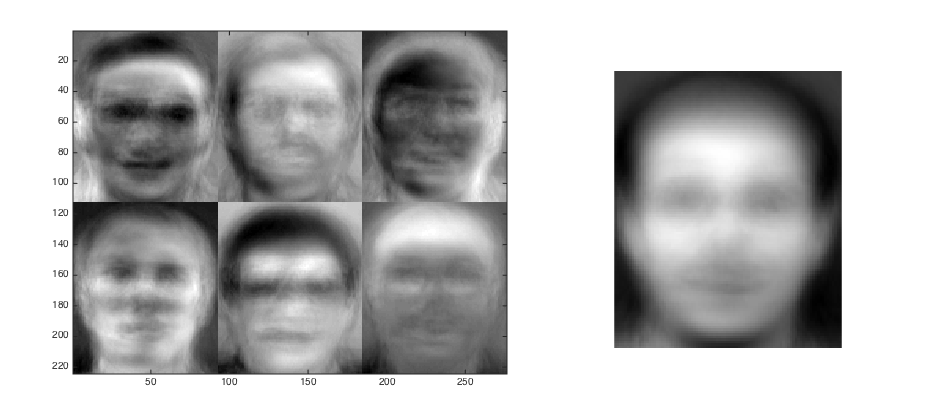
\includegraphics[width=\MyFactor\textwidth]{Img/pca_eigenspace.png} 
\caption{前6张特征脸和平均脸}
\end{figure}
其中,PCA的计算在给出特征向量的同时,还会给出代表特征向量权重的特征值,上述6个特征值在400个特征向量空间中占据了51.4\%的权重.权重分布如下图:

\begin{figure}[!htbp]
\centering 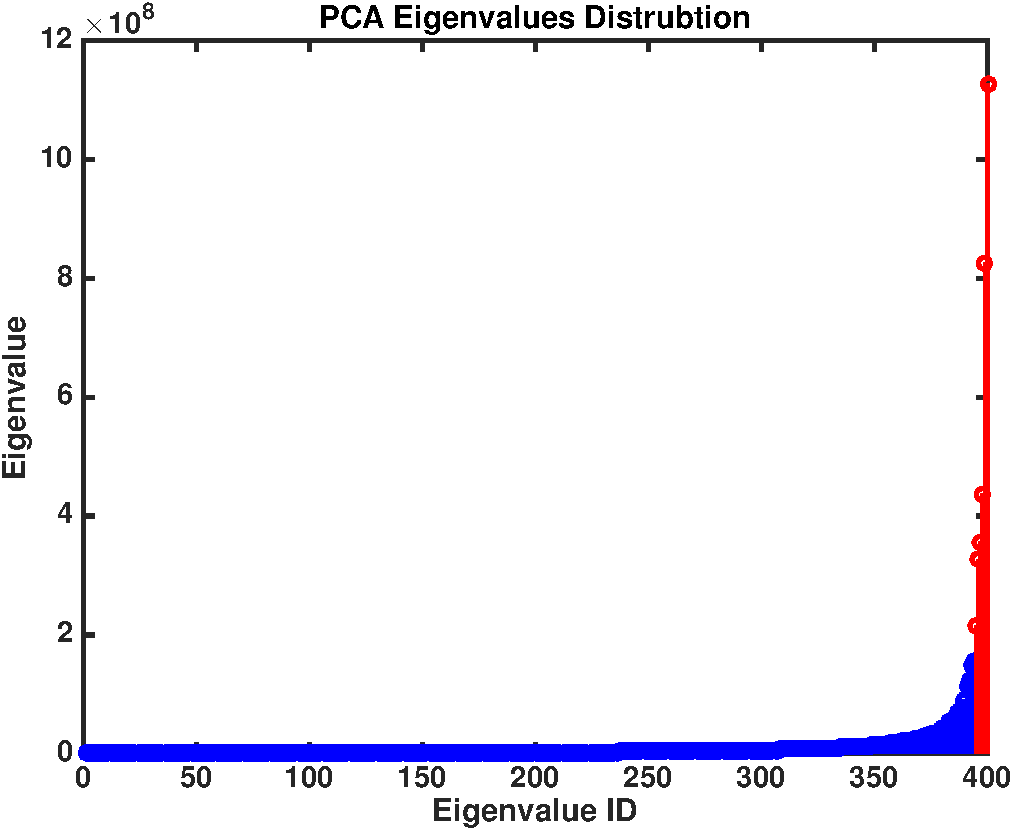
\includegraphics[width=\MyFactor\textwidth]{Img/pca_eivalue.pdf} 
\caption{特征值分布图 \\ 蓝色:舍弃的特征向量, 红色: 保留的特征向量}
\end{figure}



\paragraph{输入样本投影} 这一步骤是将
\paragraph{输入样本重构}
\section{PCA}
\section{NMF}
\section{ICA}